\chapter{The surrogate problem and the toolkit}
\label{ch:toolkit}

This chapter sets up the problem the whole book is about and builds the tools every later chapter uses: geometry of
vectors and functions, the few matrix facts that do all the work, least squares, the numerical facts that decide
whether a computation can be trusted, probability done with integrals, and the multivariate Gaussian. It ends with
Bayesian linear regression, which turns out to be a Gaussian process in disguise; Chapter~2 removes the disguise.

\section{What a surrogate is}

You have a function you can evaluate but not afford to evaluate often: a finite-element run, a CFD solve, a
wind-tunnel test. Write it as
\begin{equation}
  f : \mathcal{X} \to \R, \qquad \mathcal{X} \subset \R^d ,
\end{equation}
where $x \in \mathcal{X}$ collects the $d$ design inputs (geometry parameters, operating conditions) and $f(x)$ is
the output you care about. We assume, after rescaling, that $\mathcal{X} = [0,1]^d$, the unit cube; every learner in
the study works on this cube.

You run the simulator at $n$ chosen inputs $x_1, \dots, x_n$ (the \emph{design}) and record
\begin{equation}
  y_i = f(x_i) + \varepsilon_i , \qquad i = 1, \dots, n,
  \label{eq:data}
\end{equation}
where $\varepsilon_i$ is noise: solver tolerance, mesh effects, stochastic physics, measurement error. For an exact
deterministic code $\varepsilon_i = 0$. The data set is $\mathcal{D} = \{(x_i, y_i)\}_{i=1}^n$.

\begin{definition}[Surrogate]
A surrogate is a function $\hat f : \mathcal{X} \to \R$ built from $\mathcal{D}$ that is cheap to evaluate and
stands in for $f$.
\end{definition}

A surrogate is used for one of three jobs, and they want different things:
\begin{enumerate}[nosep]
  \item \textbf{Prediction}: $\hat f(x) \approx f(x)$ everywhere in $\mathcal{X}$. Measured by an average error.
  \item \textbf{Optimisation}: the minimiser of $\hat f$ should be a good design for $f$. Only the region near the
        optimum matters, and an optimiser that uses gradients also needs $\nabla \hat f \approx \nabla f$ there.
  \item \textbf{Uncertainty quantification}: statements like ``$f(x)$ lies in this interval with 95\% probability'',
        or averages of $f$ over uncertain inputs. Needs an honest error estimate, not just a good guess.
\end{enumerate}
The paper's central claim is that the most accurate surrogate for job 1 need not be the best for job 2. This book
supplies the mathematics to see why.

\begin{intuition}
Every surrogate method is an answer to one question: \emph{which functions do you believe $f$ could be?} With $n$
numbers you cannot pin down a function on a continuum; infinitely many functions pass through any data. A method
picks one by preferring some functions over others: smooth ones (Gaussian processes, splines), piecewise-constant
ones (trees), sums of simple pieces (additive models), ratios of polynomials (rational methods). This preference is
called the \emph{inductive bias}. A method wins exactly when its preference matches the truth.
\end{intuition}

\section{Why the problem is hard: dimension and smoothness}
\label{sec:curse}

\paragraph{Grids explode.} Ten samples per input is a modest resolution. In $d$ dimensions a grid needs $10^d$
points: 100 for $d = 2$, $10^5$ for $d = 5$, $10^{10}$ for $d = 10$. At one CPU-hour per finite-element run, $d = 5$
already costs eleven years.

\paragraph{Space becomes empty and corner-heavy.} Inscribe a ball of radius $\tfrac12$ in the unit cube. The share of
the cube's volume inside the ball is $0.785$ for $d = 2$, $0.164$ for $d = 5$, $0.0025$ for $d = 10$ and
$2.5\times 10^{-8}$ for $d = 20$. In high dimension almost all the volume is in the corners, far from the centre, so
almost every new point is far from every sample.

\paragraph{Distances stop discriminating.} Take 1000 random points in the cube and a random query point. The ratio
(largest distance $-$ smallest distance)/smallest distance is about 135 for $d = 2$ but only 3.5 for $d = 10$ and
0.39 for $d = 100$. Methods that weight data by distance (nearest neighbours, inverse-distance weighting, kernels
with one length-scale) lose their footing, because ``near'' and ``far'' become nearly the same.

\paragraph{How fast can error fall?} Suppose $f$ is smooth in the sense that its first $s$ derivatives exist and are
bounded. Near any point, $f$ is then matched by its Taylor polynomial of degree $s-1$ with an error proportional to
$h^s$, where $h$ is the distance to the nearest sample. Spread $n$ points evenly in $d$ dimensions and each one
owns a cell of volume about $1/n$, so cells have side $h \approx n^{-1/d}$. Putting these together,
\begin{equation}
  \text{error} \;\approx\; C\, h^{s} \;\approx\; C\, n^{-s/d},
  \qquad\text{so}\qquad
  n \;\approx\; (C/\epsilon)^{d/s} \text{ samples for error } \epsilon .
  \label{eq:rate}
\end{equation}
For error $\epsilon = 0.01$ with $s = 2$ (and $C = 1$) this is 10 samples in one dimension, 100 in two and $10^{10}$
in ten. Approximation theory shows this rate is also the best any method can guarantee for the \emph{worst}
function of that smoothness, so no algorithm escapes it in general (Figure~\ref{fig:rates}).

\begin{figure}[t]
  \centering
  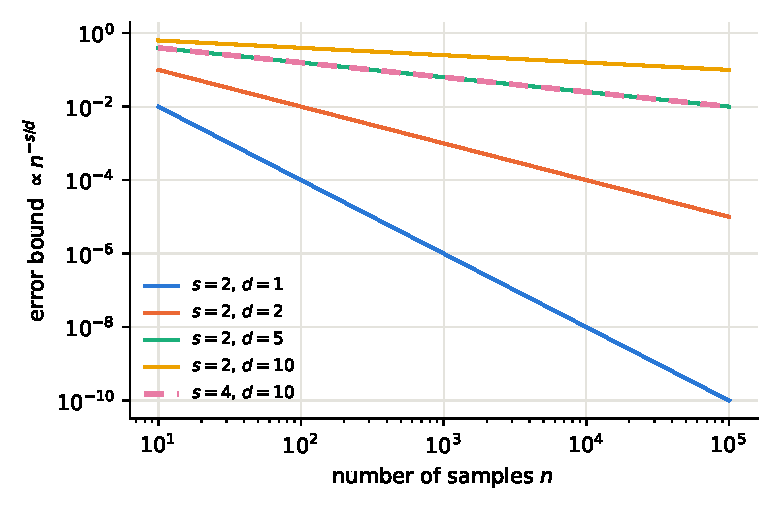
\includegraphics[width=0.62\textwidth]{figures/ch01_rates.pdf}
  \caption{The rate $n^{-s/d}$ of equation~\eqref{eq:rate}. Smoothness $s$ buys speed; dimension $d$ takes it
  away. Only the ratio $s/d$ matters: doubling the smoothness at $d = 10$ (pink, dashed) gives exactly the curve
  of halving the dimension to $d = 5$ (green, underneath it).}
  \label{fig:rates}
\end{figure}

\begin{intuition}
Equation~\eqref{eq:rate} is the single most important fact in surrogate modelling. It says three things. Smoother
functions are easier ($s$ up). Higher dimension is catastrophic ($d$ up). And the only escape is \emph{structure}:
if $f$ secretly depends on fewer effective inputs (a ridge $g(w\T x)$), is a sum of one-dimensional pieces
($\sum_j g_j(x_j)$), is low-rank ($\prod_j g_j(x_j)$), or is very smooth, then the effective $d/s$ is small. Most of
the methods in this book are ways of betting on one kind of structure.
\end{intuition}

\section{Vectors, inner products and projection}
\label{sec:vectors}

You met these in a proofs course; here each property is restated with the reason it holds, because later chapters
lean on the reasons, not the names.

\paragraph{Vector spaces and bases.} A vector space is a set where you can add elements and scale them by numbers,
and the usual rules hold. A \emph{basis} $\{v_1,\dots,v_k\}$ is a set of vectors such that every vector is a
combination $c_1 v_1 + \dots + c_k v_k$ in \emph{exactly one} way. ``At least one way'' means the basis spans the
space; ``at most one way'' means no basis vector is a combination of the others (linear independence). The numbers
$c_j$ are the \emph{coordinates}. All bases of a space have the same size, the \emph{dimension}: if one basis were
smaller, you could rewrite the larger one in terms of it and find a dependency.

\paragraph{Functions are vectors.} Functions on $[0,1]^d$ add and scale pointwise, so they form a vector space. The
polynomials of degree at most $p$ in one variable have basis $1, t, t^2, \dots, t^p$, so dimension $p+1$. Fitting a
surrogate is choosing coordinates in some space of functions. The space of \emph{all} functions has no finite basis,
which is why every method restricts itself somehow.

\begin{definition}[Inner product and norm]
An inner product $\ip{u}{v}$ is a way to multiply two vectors to a number that is symmetric
($\ip{u}{v} = \ip{v}{u}$), linear in each argument, and positive ($\ip{u}{u} > 0$ for $u \neq 0$). It defines a
length $\norm{u} = \sqrt{\ip{u}{u}}$ and an angle. In $\R^n$: $\ip{u}{v} = u\T v = \sum_i u_i v_i$. For functions on
$[0,1]$:
\begin{equation}
  \ip{g}{h} = \int_0^1 g(t)\, h(t)\, dt, \qquad \norm{g}^2 = \int_0^1 g(t)^2\, dt ,
\end{equation}
so the ``length'' of a function is its root-mean-square size. A surrogate's mean-squared error is the squared
length $\norm{\hat f - f}^2$ of the error function.
\end{definition}

\begin{result}[Cauchy--Schwarz]
$|\ip{u}{v}| \le \norm{u}\,\norm{v}$, with equality only when $u$ and $v$ are parallel.
\end{result}
\begin{intuition}
For every number $t$, the squared length $\norm{u - t v}^2 = \norm{u}^2 - 2t\ip{u}{v} + t^2\norm{v}^2$ is at least
zero. A quadratic in $t$ that is never negative cannot have two real roots, so its discriminant
$4\ip{u}{v}^2 - 4\norm{u}^2\norm{v}^2$ is not positive. That is the inequality. It is what lets us define the angle
$\cos\theta = \ip{u}{v}/(\norm{u}\norm{v})$: the ratio is guaranteed to lie in $[-1,1]$.
\end{intuition}

\paragraph{Orthogonality and Gram--Schmidt.} Vectors are orthogonal when $\ip{u}{v} = 0$. An orthonormal basis
$\{e_j\}$ (orthogonal, unit length) makes coordinates trivial: the coordinate of $u$ along $e_j$ is just
$\ip{u}{e_j}$, because taking the inner product of $u = \sum_k c_k e_k$ with $e_j$ kills every term except
$c_j$. Gram--Schmidt turns any basis $v_1, v_2, \dots$ into an orthonormal one:
\begin{equation}
  u_k = v_k - \sum_{j<k} \ip{v_k}{e_j}\, e_j, \qquad e_k = u_k / \norm{u_k}.
\end{equation}
\emph{Why it works:} $\ip{v_k}{e_j}\, e_j$ is the part of $v_k$ that points along $e_j$; subtracting all those parts
leaves only the genuinely new direction. Applied to $1, t, t^2, \dots$ on $[-1,1]$ with the integral inner product,
Gram--Schmidt produces (up to scaling) the \emph{Legendre polynomials} $P_0 = 1$, $P_1 = t$,
$P_2 = \tfrac12(3t^2-1), \dots$ --- an orthogonal basis of polynomials. Section~\ref{sec:numerics} shows why that
matters numerically.

\begin{result}[Orthogonal projection]
\label{res:projection}
Let $S$ be a subspace and $y$ any vector. There is exactly one $p \in S$ closest to $y$, and it is characterised by
the residual being orthogonal to the whole subspace: $\ip{y - p}{s} = 0$ for every $s \in S$.
If $\{e_j\}$ is an orthonormal basis of $S$, then $p = \sum_j \ip{y}{e_j}\, e_j$.
\end{result}
\begin{intuition}
Pythagoras. Suppose $y - p$ is orthogonal to $S$, and take any other $s \in S$. Then $p - s$ lies in $S$, so it is
orthogonal to $y - p$, and
\[
  \norm{y - s}^2 = \norm{(y - p) + (p - s)}^2 = \norm{y-p}^2 + \norm{p-s}^2 \;\ge\; \norm{y - p}^2 .
\]
Any other candidate is farther away by exactly the extra leg $\norm{p - s}$. The closest point is the foot of the
perpendicular, just as in the plane.
\end{intuition}

\begin{connection}
POD is projection. You collect snapshots of a flow field as columns of a matrix, find an orthonormal basis (the POD
modes) of a low-dimensional subspace, and represent each snapshot by its projection $\sum_j \ip{u}{e_j}\, e_j$. The
POD modes are chosen so that, averaged over the snapshots, the projection error is as small as possible for that
number of modes (Result~\ref{res:eckart} below). Least-squares fitting, Galerkin methods and Gaussian-process
prediction are all projections in suitably chosen spaces.
\end{connection}

\section{The matrices that matter}

\paragraph{Symmetric matrices.} A matrix is symmetric when $A = A\T$. Covariance matrices, Gram matrices $A\T A$ and
kernel matrices are all symmetric, so this case dominates the book.

\begin{result}[Spectral theorem]
A real symmetric $n\times n$ matrix has $n$ real eigenvalues and an orthonormal basis of eigenvectors:
$A = Q \Lambda Q\T$, where $Q$ has the eigenvectors as columns ($Q\T Q = I$) and $\Lambda$ is diagonal.
\end{result}
\begin{intuition}
Two eigenvectors with different eigenvalues are automatically orthogonal: if $Av_1 = \lambda_1 v_1$ and
$Av_2 = \lambda_2 v_2$, then
$\lambda_1 \ip{v_1}{v_2} = \ip{Av_1}{v_2} = \ip{v_1}{Av_2} = \lambda_2 \ip{v_1}{v_2}$, using symmetry in the
middle step. With $\lambda_1 \ne \lambda_2$ that forces $\ip{v_1}{v_2} = 0$. Geometrically, a symmetric matrix
does nothing but stretch space along perpendicular axes: in the coordinates of its eigenvectors it is a diagonal
scaling.
\end{intuition}

\begin{definition}[Positive (semi)definite]
A symmetric $A$ is positive definite (PD) if $x\T A x > 0$ for every $x \ne 0$, and positive semidefinite (PSD) if
$x\T A x \ge 0$. Write $x = Q c$ in eigen-coordinates; then $x\T A x = \sum_i \lambda_i c_i^2$, so
\emph{PD $\iff$ all eigenvalues positive} and \emph{PSD $\iff$ all eigenvalues nonnegative}.
\end{definition}
The quantity $x\T A x$ is like an energy: PD means every direction costs energy. Two facts carry most of the weight
later:
\begin{itemize}[nosep]
  \item \textbf{Gram matrices are PSD.} For any matrix $\Phi$, $x\T(\Phi\T\Phi)x = \norm{\Phi x}^2 \ge 0$. They are
        PD exactly when $\Phi$ has independent columns (otherwise some $x \ne 0$ has $\Phi x = 0$).
  \item \textbf{Covariance matrices are PSD.} $\Var(a\T X) = a\T \Cov(X)\, a \ge 0$ because a variance cannot be
        negative (Section~\ref{sec:prob}).
\end{itemize}

\begin{result}[Singular value decomposition]
Every $m \times n$ matrix factors as $A = U \Sigma V\T$ with $U$ ($m\times m$) and $V$ ($n\times n$) orthogonal and
$\Sigma$ diagonal with entries $\sigma_1 \ge \sigma_2 \ge \dots \ge 0$, the singular values. Equivalently
$A v_j = \sigma_j u_j$: $A$ sends the orthonormal directions $v_j$ to the orthonormal directions $u_j$, stretched by
$\sigma_j$.
\end{result}
\begin{intuition}
Any matrix is rotate, stretch, rotate. The right singular vectors $v_j$ are the eigenvectors of the symmetric PSD
matrix $A\T A$ (so they exist by the spectral theorem), and $\sigma_j^2$ are its eigenvalues; then
$u_j = A v_j/\sigma_j$ come out orthonormal automatically. The number of nonzero $\sigma_j$ is the rank: how many
independent directions $A$ really uses.
\end{intuition}

\begin{result}[Best low-rank approximation, Eckart--Young]
\label{res:eckart}
Keeping the first $k$ terms, $A_k = \sum_{j\le k} \sigma_j u_j v_j\T$, gives the closest rank-$k$ matrix to $A$,
and the squared error is $\sum_{j>k} \sigma_j^2$.
\end{result}
\begin{connection}
This is POD. With snapshots as columns of $A$, the left singular vectors $u_j$ are the POD modes, $\sigma_j^2$ is the
``energy'' each mode captures, and truncating at $k$ modes is optimal in the least-squares sense with the discarded
energy as the error. DMD starts from exactly this truncated SVD of the snapshot matrix before fitting its linear
operator. The low-rank surrogates of later chapters (functional SVD, tensor trains) are the same idea applied to a
function of several variables instead of a snapshot matrix.
\end{connection}

\section{Least squares}
\label{sec:ls}

Most surrogates contain a least-squares problem. Choose basis functions $\phi_1, \dots, \phi_k$ (monomials, Legendre
polynomials, radial functions\dots) and look for $\hat f(x) = \sum_j w_j \phi_j(x)$. Collect $\Phi_{ij} =
\phi_j(x_i)$ in the $n\times k$ \emph{design matrix} and solve
\begin{equation}
  \min_{w \in \R^k} \norm{y - \Phi w}^2 = \min_w \sum_{i=1}^n \Big(y_i - \sum_j w_j \phi_j(x_i)\Big)^2 .
\end{equation}
The vectors $\Phi w$ form a subspace of $\R^n$ (the column space of $\Phi$), so this is projecting $y$ onto it.
By Result~\ref{res:projection} the residual must be orthogonal to every column:
\begin{equation}
  \Phi\T (y - \Phi w) = 0 \quad\Longleftrightarrow\quad \Phi\T\Phi\, w = \Phi\T y .
  \label{eq:normal}
\end{equation}
These are the \emph{normal equations}. They have a unique solution exactly when the columns are independent (the
Gram matrix $\Phi\T\Phi$ is then PD, hence invertible).

With the SVD $\Phi = U \Sigma V\T$ (thin form, $\sigma_j > 0$),
\begin{equation}
  w = V \Sigma^{-1} U\T y = \sum_j \frac{u_j\T y}{\sigma_j}\, v_j .
  \label{eq:ls_svd}
\end{equation}
Read it as: express $y$ in the output directions $u_j$, divide by how much $\Phi$ stretches each direction, and map
back. The danger is visible already: a tiny $\sigma_j$ divides, so any noise in $y$ along $u_j$ is blown up.

\begin{connection}
DMD's best-fit linear operator, $X' \approx A X$, is a least-squares problem of exactly this type, and ``exact DMD''
solves it through the truncated SVD of $X$, discarding small $\sigma_j$ for exactly the reason above.
\end{connection}

\section{Numerical facts that decide what can be trusted}
\label{sec:numerics}

\paragraph{Floating point.} A computer stores a real number $x$ as $\mathrm{fl}(x) = x(1 + \delta)$ with
$|\delta| \le u$, the \emph{unit round-off}; for standard double precision $u = 2^{-53} \approx 1.1 \times
10^{-16}$. Every arithmetic operation adds such a relative error. This is harmless until two nearly equal numbers are
subtracted: the leading digits cancel and only the rounding errors are left (\emph{cancellation}).

\paragraph{Conditioning.} A problem is \emph{ill-conditioned} if small changes in its data cause large changes in its
answer, whatever algorithm you use. For a square linear system $Aw = b$ the amplification factor is the
\emph{condition number}
\begin{equation}
  \kappa(A) = \frac{\sigma_{\max}}{\sigma_{\min}},
  \qquad
  \frac{\norm{\delta w}}{\norm{w}} \;\lesssim\; \kappa(A)\, \frac{\norm{\delta b}}{\norm{b}} .
\end{equation}
\emph{Why:} by \eqref{eq:ls_svd} a perturbation of $b$ along the weakest direction is divided by $\sigma_{\min}$,
while $b$ itself can lie along the strongest one. Rule of thumb: you lose about $\log_{10}\kappa$ of your 16 digits.

\begin{example}[Bases matter]
Fit polynomials of degree $p$ on $[-1,1]$ from 100 equally spaced points. Condition numbers of the design matrix:
\begin{center}
\begin{tabular}{lrrr}
\toprule
degree $p$ & monomials $1,t,\dots,t^p$ & Legendre $P_0,\dots,P_p$ & normal equations, monomials \\
\midrule
5  & $4.2\times10^{1}$ & 3.2 & $1.8\times10^{3}$ \\
10 & $2.9\times10^{3}$ & 4.4 & $8.6\times10^{6}$ \\
15 & $2.2\times10^{5}$ & 5.5 & $4.8\times10^{10}$ \\
20 & $1.7\times10^{7}$ & 6.4 & $3.0\times10^{14}$ \\
\bottomrule
\end{tabular}
\end{center}
The function space is identical; only the basis differs. Monomials $t^{15}$ and $t^{17}$ look almost the same on
$[-1,1]$ (nearly parallel vectors), so separating them is ill-conditioned; Legendre polynomials are orthogonal, so
nothing needs separating. The last column shows the second lesson: forming $\Phi\T\Phi$ squares the condition
number ($\kappa(\Phi\T\Phi) = \kappa(\Phi)^2$, since its singular values are $\sigma_j^2$). At degree 20 that leaves
two correct digits. Solve least squares through QR or the SVD, never by forming the normal equations.
\end{example}

\paragraph{Stability.} Conditioning belongs to the problem; \emph{stability} belongs to the algorithm. A stable
algorithm gives an answer as accurate as the conditioning allows. Forming $\Phi\T\Phi$ is an unstable route to a
least-squares solution (it squares $\kappa$ before solving); QR is a stable one.

\paragraph{Cholesky, and why we never invert.} A PD matrix factors uniquely as $A = L L\T$ with $L$ lower
triangular (\emph{Cholesky}). It exists because positivity guarantees every pivot is positive, so the square roots
in the construction are real. It costs $n^3/3$ operations, half of a general factorisation. To solve $Aw = b$, solve
$Lz = b$ then $L\T w = z$, each by substitution in $n^2$ operations. Two by-products appear constantly in
Gaussian-process work: $\log\det A = 2\sum_i \log L_{ii}$ (stable, never overflows), and a cheap test of whether
$A$ is numerically PD (the factorisation fails if not). Computing $A^{-1}$ explicitly costs more and is less
accurate than solving; ``$A^{-1}b$'' in a formula always means ``solve''.

\paragraph{Finite differences: the trade-off you asked about.} To approximate $f'(x)$ by
$\big(f(x+h) - f(x)\big)/h$ there are two errors. Taylor's theorem gives a truncation error of about
$\tfrac{h}{2}|f''|$, which shrinks with $h$. Rounding gives about $2u|f|/h$, which grows as $h$ shrinks, because
$f(x+h) - f(x)$ is a cancellation. The total is smallest when the two balance, at $h \approx \sqrt{u} \approx
10^{-8}$, leaving about $10^{-8}$ error. The central difference $\big(f(x+h) - f(x-h)\big)/(2h)$ has truncation
error $\tfrac{h^2}{6}|f'''|$; balancing against $u|f|/h$ gives $h \approx u^{1/3} \approx 5\times10^{-6}$ and an
error near $10^{-11}$. Figure~\ref{fig:fd} shows both for $f = \sin$ at $x = 1$: the V shapes are exactly this
trade-off.

\begin{figure}[t]
  \centering
  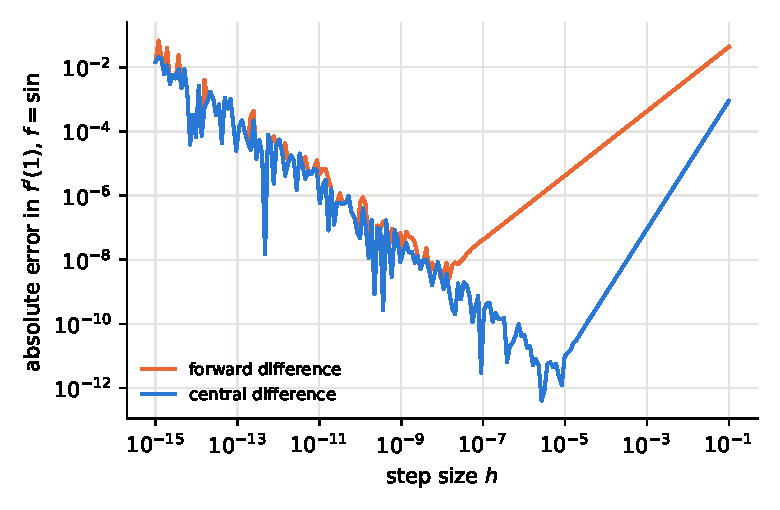
\includegraphics[width=0.62\textwidth]{figures/ch01_fd_error.pdf}
  \caption{Finite-difference error versus step size for $f'(1)$, $f = \sin$. Right of each minimum, truncation
  error dominates (slope 1 forward, slope 2 central); left of it, rounding dominates (slope $-1$). The study's
  gradient metric uses central differences with $h = 10^{-5}$, near the bottom of the blue V.}
  \label{fig:fd}
\end{figure}

\begin{pitfall}
The finite-difference error that matters in practice is not this one. An optimizer differencing a surrogate with a
practitioner's step ($10^{-3}$, say) across a kink, a jump or a noisy surface gets an error unrelated to round-off.
That is why the study measures gradient accuracy with a tiny, accurate step, and treats the optimizer's own
gradient source as a separate factor in the optimisation experiment.
\end{pitfall}

\section{Regularisation: trading a little bias for stability}
\label{sec:ridge}

When $\Phi$ has small singular values, \eqref{eq:ls_svd} amplifies noise. \emph{Ridge regression} (Tikhonov
regularisation) adds a penalty:
\begin{equation}
  \min_w \; \norm{y - \Phi w}^2 + \lambda \norm{w}^2
  \quad\Longrightarrow\quad
  (\Phi\T\Phi + \lambda I)\, w = \Phi\T y
  \quad\Longrightarrow\quad
  w = \sum_j \frac{\sigma_j}{\sigma_j^2 + \lambda}\, (u_j\T y)\, v_j .
  \label{eq:ridge}
\end{equation}
Compare with \eqref{eq:ls_svd}: the factor $1/\sigma_j$ has become $\sigma_j/(\sigma_j^2+\lambda)$. For strong
directions ($\sigma_j^2 \gg \lambda$) nothing changes; for weak ones ($\sigma_j^2 \ll \lambda$) the factor is about
$\sigma_j/\lambda$, which goes to zero instead of blowing up. Ridge is a smooth version of throwing away small
singular values, the ``filter factors'' $\sigma_j^2/(\sigma_j^2+\lambda)$ that you may know from POD-based
reduced-order models. The price is \emph{bias}: even with perfect data, $w$ is pulled towards zero. Choosing $\lambda$
is choosing how much bias to accept for how much stability; Section~\ref{sec:estimation} makes this exact.

Every regularised method later in the book --- the GP nugget, the Tikhonov denominator of rational fits, the ridge
inside alternating least squares --- is this same filter in a different basis.

\section{Probability with integrals}
\label{sec:prob}

Statistics courses often switch to tables early. Here everything is an integral, and the tables are explained at
the end as what they are.

\begin{definition}[Density]
A continuous random variable $X$ is described by a density $p(x) \ge 0$ with $\int p(x)\,dx = 1$. Probabilities are
areas under it:
\begin{equation}
  \Pr(a \le X \le b) = \int_a^b p(x)\, dx .
\end{equation}
The density is not a probability; it is probability per unit length. It can exceed 1; only its integral is bounded.
\end{definition}

\paragraph{Expectation, mean, variance.} The expected value of any function $g$ of $X$ is a weighted average:
\begin{equation}
  \E[g(X)] = \int g(x)\, p(x)\, dx .
\end{equation}
The mean is $\mu = \E[X]$, the variance $\Var(X) = \E[(X - \mu)^2]$, and the standard deviation $\sqrt{\Var X}$.
Expanding the square and using linearity of the integral, $\Var(X) = \E[X^2] - \mu^2$. Linearity is the property
used most: $\E[aX + bY] = a\E[X] + b\E[Y]$ always, because an integral of a sum is the sum of integrals.

\paragraph{Several variables.} Two variables have a joint density $p(x, y)$, with $\Pr\big((X,Y) \in R\big) =
\iint_R p(x,y)\,dx\,dy$. Three operations do everything:
\begin{itemize}[nosep]
  \item \textbf{Marginalise} (forget $y$): $p(x) = \int p(x, y)\, dy$. Integrate out what you do not care about.
  \item \textbf{Condition} (learn that $X = x$): $p(y \mid x) = p(x, y)/p(x)$. Take the slice of the joint density at
        $X = x$ and rescale it so it integrates to one; the divisor is exactly the marginal.
  \item \textbf{Bayes' rule}: writing the joint both ways, $p(x,y) = p(y\mid x)\,p(x) = p(x\mid y)\,p(y)$, gives
        \begin{equation}
          p(\theta \mid \mathcal{D}) = \frac{p(\mathcal{D} \mid \theta)\; p(\theta)}{p(\mathcal{D})},
          \qquad p(\mathcal{D}) = \int p(\mathcal{D}\mid\theta)\,p(\theta)\,d\theta .
          \label{eq:bayes}
        \end{equation}
\end{itemize}
In words: what you believe about unknowns $\theta$ after seeing data (the \emph{posterior}) is what you believed
before (the \emph{prior}) times how well each $\theta$ explains the data (the \emph{likelihood}), rescaled to integrate
to one. Nothing more is going on in any Bayesian method in this book.

\paragraph{Independence and covariance.} $X$ and $Y$ are independent when $p(x,y) = p(x)\,p(y)$: learning one tells
you nothing about the other. Their covariance is $\Cov(X,Y) = \E[(X - \mu_X)(Y - \mu_Y)]$, which measures linear
co-movement. For a vector $X$, the covariance matrix has entries $\Cov(X_i, X_j)$, and for any fixed vector $a$,
$\Var(a\T X) = a\T \Cov(X)\, a$ --- which is why covariance matrices are PSD.

\begin{connection}[What a statistical table is]
A ``$z$-table'' lists $\Phi(z) = \int_{-\infty}^{z} \frac{1}{\sqrt{2\pi}} e^{-t^2/2}\,dt$ for many $z$: the area
under the standard bell curve to the left of $z$. This integral has no formula in elementary functions, so it was
computed numerically once and printed. ``Look up 1.96 in the table'' means ``the area to the left of 1.96 is
0.975'', so the central area between $-1.96$ and $1.96$ is 0.95: that is where 95\% intervals come from. $t$-tables
and $\chi^2$-tables are the same thing for other densities. Today one calls \texttt{scipy.stats.norm.cdf}.
\end{connection}

\section{The multivariate Gaussian}
\label{sec:gauss}

\begin{definition}[Gaussian distribution]
$X \in \R^d$ is Gaussian with mean $\mu$ and covariance $\Sigma$ (PD), written $X \sim \N(\mu, \Sigma)$, if
\begin{equation}
  p(x) = \frac{1}{(2\pi)^{d/2}\, \det(\Sigma)^{1/2}}
  \exp\!\Big(-\tfrac12 (x - \mu)\T \Sigma^{-1} (x - \mu)\Big).
  \label{eq:gauss}
\end{equation}
\end{definition}
\paragraph{Reading the formula.} The exponent contains $(x-\mu)\T\Sigma^{-1}(x-\mu)$, a squared distance from the mean
measured in units of the spread: the \emph{Mahalanobis distance}. In the eigenvector coordinates of $\Sigma$ (spectral
theorem) it becomes $\sum_i c_i^2/\lambda_i$: each direction is measured relative to its own variance $\lambda_i$, so
the level sets are ellipsoids with axes along the eigenvectors and half-lengths $\sqrt{\lambda_i}$. In those same
coordinates the density is a product of $d$ one-dimensional bell curves, each integrating to $\sqrt{2\pi\lambda_i}$;
the product is $(2\pi)^{d/2}\prod_i\sqrt{\lambda_i} = (2\pi)^{d/2}\det(\Sigma)^{1/2}$, which is the normalising
constant. Nothing in \eqref{eq:gauss} is arbitrary.

Four properties make Gaussians the workhorse of uncertainty quantification.
\begin{result}[Linear maps preserve Gaussianity]
If $X \sim \N(\mu,\Sigma)$ then $AX + b \sim \N(A\mu + b,\; A\Sigma A\T)$.
\end{result}
\emph{Why:} the mean and covariance follow from linearity of expectation; Gaussianity survives because substituting
a linear change of variables into a quadratic exponent leaves a quadratic exponent. In particular a sum of jointly
Gaussian variables is Gaussian, so a prediction that is a weighted sum of Gaussian unknowns is Gaussian too.

\begin{result}[Marginals]
Split $X = (a, b)$ with $\mu = (\mu_a, \mu_b)$ and $\Sigma = \begin{psmallmatrix}\Sigma_{aa} &
\Sigma_{ab}\\ \Sigma_{ba} & \Sigma_{bb}\end{psmallmatrix}$. Then $a \sim \N(\mu_a, \Sigma_{aa})$: to forget $b$,
delete its rows and columns. (This is the linear map that picks out $a$.)
\end{result}

\begin{result}[Uncorrelated means independent, for Gaussians]
If $\Sigma_{ab} = 0$, then $a$ and $b$ are independent.
\end{result}
\emph{Why:} with a block-diagonal $\Sigma$, the inverse is block diagonal and the exponent splits as a sum of an
$a$-part and a $b$-part, so the density factorises. (For non-Gaussian variables, zero covariance does \emph{not}
imply independence.)

\begin{result}[Conditioning --- the engine of Gaussian-process prediction]
\label{res:condition}
For $(a, b)$ jointly Gaussian as above,
\begin{equation}
  a \mid b \;\sim\; \N\!\Big(\mu_a + \Sigma_{ab}\Sigma_{bb}^{-1}(b - \mu_b),\;\;
                           \Sigma_{aa} - \Sigma_{ab}\Sigma_{bb}^{-1}\Sigma_{ba}\Big).
  \label{eq:condition}
\end{equation}
\end{result}
\begin{intuition}
Remove from $a$ the part that $b$ can explain linearly. Define $z = a - \Sigma_{ab}\Sigma_{bb}^{-1} b$. Its
covariance with $b$ is $\Sigma_{ab} - \Sigma_{ab}\Sigma_{bb}^{-1}\Sigma_{bb} = 0$, and $(z, b)$ is jointly Gaussian
(a linear map of $(a,b)$), so by the previous result $z$ is \emph{independent} of $b$. Now write
$a = z + \Sigma_{ab}\Sigma_{bb}^{-1} b$. Once $b$ is known, the second term is a known constant and $z$ keeps its
own distribution, because it does not care about $b$. So $a \mid b$ has mean
$\E[z] + \Sigma_{ab}\Sigma_{bb}^{-1}b = \mu_a + \Sigma_{ab}\Sigma_{bb}^{-1}(b - \mu_b)$ and covariance $\Cov(z) =
\Sigma_{aa} - \Sigma_{ab}\Sigma_{bb}^{-1}\Sigma_{ba}$ (expand $\Cov(z)$ to check). The mean shifts by a regression
on the surprise $b - \mu_b$; the covariance shrinks by the part $b$ explains, and it does not depend on the value of
$b$ at all.
\end{intuition}

\begin{connection}
Chapter~2 applies \eqref{eq:condition} with $b$ = the observed outputs and $a$ = the unknown output at a new point.
The ``GP posterior mean and variance'' are nothing but this formula. Numerically, $\Sigma_{bb}^{-1}$ is never formed:
one Cholesky factorisation of $\Sigma_{bb}$ serves both the mean and the variance.
\end{connection}

\section{Estimation and learning}
\label{sec:estimation}

\paragraph{Estimators, bias and variance.} An estimator $\hat\theta$ is a recipe that turns data into a guess of an
unknown $\theta$. Because the data are random (noise, random design), $\hat\theta$ is a random variable. Its
mean-squared error splits exactly into two parts:
\begin{equation}
  \E\big[(\hat\theta - \theta)^2\big]
  = \underbrace{\big(\E[\hat\theta] - \theta\big)^2}_{\text{bias}^2}
  + \underbrace{\E\big[(\hat\theta - \E\hat\theta)^2\big]}_{\text{variance}} .
  \label{eq:biasvar}
\end{equation}
\emph{Why:} add and subtract $\E[\hat\theta]$ inside the square; the cross term has expectation zero because
$\E[\hat\theta - \E\hat\theta] = 0$. Bias is being wrong on average; variance is being unstable from one data set to
the next. Ridge regression accepts bias to cut variance; a very flexible model has low bias and high variance. A
surrogate's error behaves the same way at every point $x$.

\paragraph{Maximum likelihood is least squares.} Assume the noise in \eqref{eq:data} is independent Gaussian with
variance $\sigma^2$ and $f(x) = \phi(x)\T w$. The likelihood of the data is the product of the individual densities,
\begin{equation}
  p(y \mid w) = \prod_{i=1}^n \frac{1}{\sqrt{2\pi\sigma^2}}
  \exp\!\Big(-\frac{(y_i - \phi(x_i)\T w)^2}{2\sigma^2}\Big),
  \qquad
  -\log p(y\mid w) = \frac{1}{2\sigma^2}\norm{y - \Phi w}^2 + \text{const}.
\end{equation}
Maximising the likelihood is therefore exactly least squares. Least squares is the right fit for Gaussian noise; for
heavy-tailed noise (occasional outliers) other losses fit better, which is part of why some methods do better under
the study's heavy-tailed noise condition.

\paragraph{Maximum a posteriori is ridge.} Add a prior belief that weights are modest: $w \sim \N(0, \tau^2 I)$.
By Bayes' rule \eqref{eq:bayes}, the log posterior is the log likelihood plus the log prior:
\begin{equation}
  -\log p(w \mid y) = \frac{1}{2\sigma^2}\norm{y - \Phi w}^2 + \frac{1}{2\tau^2}\norm{w}^2 + \text{const}.
\end{equation}
Its minimiser is ridge regression \eqref{eq:ridge} with $\lambda = \sigma^2/\tau^2$: noise level over prior size.
Regularisation is not a trick; it is a prior belief written as a penalty.

\paragraph{Bayesian linear regression: the whole posterior.} Instead of the single best $w$, keep the full posterior.
Treat $w$ and $y = \Phi w + \varepsilon$ as jointly Gaussian. By the linear-map rule, $y \sim \N(0,\; \tau^2\Phi\Phi\T
+ \sigma^2 I)$ and $\Cov(w, y) = \tau^2\Phi\T$. Conditioning \eqref{eq:condition} on the observed $y$ gives
\begin{equation}
  w \mid y \sim \N(m, S), \qquad
  m = \tau^2 \Phi\T\big(\tau^2 \Phi\Phi\T + \sigma^2 I\big)^{-1} y, \qquad
  S = \tau^2 I - \tau^2\Phi\T\big(\tau^2\Phi\Phi\T + \sigma^2 I\big)^{-1}\Phi\,\tau^2 .
  \label{eq:blr}
\end{equation}
A prediction at a new point, $\hat f(x_*) = \phi(x_*)\T w$, is a linear map of a Gaussian, hence Gaussian:
\begin{equation}
  \hat f(x_*) \mid y \sim \N\!\Big(\underbrace{\phi_*\T m}_{\text{prediction}},\;
                                   \underbrace{\phi_*\T S\, \phi_*}_{\text{its uncertainty}}\Big),
  \qquad \phi_* = \phi(x_*).
  \label{eq:blr_pred}
\end{equation}
Expand $\phi_*\T m = \tau^2\phi_*\T\Phi\T(\tau^2\Phi\Phi\T + \sigma^2 I)^{-1} y$. The data enter \emph{only} through
inner products $\tau^2\phi(x)\T\phi(x')$ between feature vectors: $\Phi\Phi\T$ is the matrix of those inner products
between design points, and $\Phi\phi_*$ the inner products with the new point. Call this
$k(x, x') = \tau^2\phi(x)\T\phi(x')$. Then
\begin{equation}
  \text{mean}(x_*) = k_*\T (K + \sigma^2 I)^{-1} y, \qquad
  \text{variance}(x_*) = k(x_*,x_*) - k_*\T (K + \sigma^2 I)^{-1} k_*,
  \label{eq:gp_preview}
\end{equation}
with $K_{ij} = k(x_i, x_j)$ and $(k_*)_i = k(x_i, x_*)$. This is a Gaussian process with kernel $k$. Chapter~2
starts here and asks: what if we choose $k$ directly, so that the feature space is infinite-dimensional and we never
write $\phi$ down?

\section{Measuring a surrogate}
\label{sec:measure}

The quantity we want is the true average error over the domain,
\begin{equation}
  \text{MSE}(\hat f) = \int_{\mathcal{X}} \big(\hat f(x) - f(x)\big)^2\, dx = \norm{\hat f - f}^2 .
\end{equation}
It is an integral, so we estimate it the way any integral is estimated: average the integrand at many points. The
study uses 4096 quasi-random test points and reports
\begin{equation}
  \text{NRMSE} = \frac{\sqrt{\tfrac{1}{N}\sum_{t=1}^N \big(\hat f(x_t) - f(x_t)\big)^2}}{\operatorname{sd}\big(f(x_1),
  \dots, f(x_N)\big)} ,
\end{equation}
scaled so that 1 means ``no better than predicting the mean'' and 0 is perfect.

\begin{result}[Noisy tests have a floor]
If the test outputs are themselves noisy, $\tilde y_t = f(x_t) + \varepsilon_t$ with noise of variance $\sigma^2$
independent of the surrogate, then
\begin{equation}
  \E\big[(\hat f(x) - \tilde y)^2\big] = \E\big[(\hat f(x) - f(x))^2\big] + \sigma^2 .
\end{equation}
\end{result}
\emph{Why:} write $\hat f - \tilde y = (\hat f - f) - \varepsilon$, expand the square, and the cross term vanishes
because $\varepsilon$ has mean zero and is independent of $\hat f - f$. Error measured against noisy data can never
fall below the noise variance, and when every method is near that floor their differences are compressed. This is
exactly the thesis-review finding (bug B-01): scoring against noisy cross-validation folds made the GP's lead over
boosted trees look 1.2$\times$ when on clean truth it was 2.4$\times$. With a simulator we can evaluate $f$ itself, so
the study scores against clean truth.

\paragraph{Cross-validation.} Without clean test data, hold out part of the data, fit on the rest and score on the
held-out part, rotating which part is held out. It estimates the error on new data from the same distribution, noise
floor included. Choosing hyper-parameters (a ridge $\lambda$, a polynomial degree) by such a hold-out is used
throughout the study's learners.

\section{A map of what follows}

Every later chapter is one answer to ``which functions do you believe in?'' (the inductive bias), with the
mathematics that follows from it.

\begin{center}
\small
\begin{tabular}{p{3.6cm}p{5.2cm}p{4.6cm}}
\toprule
Family & Functions it prefers & Structure it exploits (Section~\ref{sec:curse}) \\
\midrule
Gaussian processes, kernels, RBF (Ch.~2) & smooth, with a smoothness set by the kernel & smoothness $s$ \\
Polynomial chaos, sparse regression & low-degree polynomials, few active terms & smoothness, sparsity \\
Splines, GAMs, MARS & piecewise polynomials; sums of 1-D pieces & additivity \\
Trees, forests, boosting & piecewise constant on boxes & axis-aligned jumps \\
Neural networks, KANs & compositions of simple functions & compositional structure \\
Ridge / active subspaces & $g(W\T x)$ with few directions & low effective dimension \\
Low-rank, tensor trains & products of 1-D functions & separability \\
Rational (AAA, p/q) & ratios of polynomials & poles, knees, resonances \\
Bayesian NNs, BART, PFNs & a prior over functions, learned or explicit & whatever the prior encodes \\
\bottomrule
\end{tabular}
\end{center}

\section*{Notes and questions for later}
\begin{enumerate}[leftmargin=*]
  \item \textbf{Why $\mathcal{X} \subset \R^d$?} For a design study the inputs are the chosen parameters, so they
        are coordinates by construction. When the meaningful inputs lie on a lower-dimensional set (constrained
        designs, shapes, data on a manifold), nothing requires knowing that set: methods only use points and
        distances in the ambient coordinates. Embedding theorems say a representation always exists: Whitney, a
        smooth $m$-manifold embeds smoothly in $\R^{2m}$; Menger--N\"obeling, a compact space of topological dimension
        $m$ embeds continuously in $\R^{2m+1}$. Continuity is enough to embed; smoothness matters only for the
        \emph{rate} (the $s$ in $n^{-s/d}$), which drops near corners and cusps. Kernel and nearest-neighbour methods
        adapt to the intrinsic dimension $m$ (the ``manifold hypothesis''). Takens' delay embedding is the same idea
        behind delay-coordinate DMD. A later chapter on geometry and dimension treats this properly.
  \item \textbf{Why $f : \mathcal{X} \to \R$ and not $\R^n$?} A design objective is scalar. Vector and field outputs
        (independent models, multi-output GPs and co-kriging, POD coefficients plus regression, i.e.\ non-intrusive
        ROMs) get their own chapter.
  \item \textbf{Eckart--Young says how to truncate at a given $k$, not how to choose $k$.} Choosing $k$ from noisy
        data is Gavish and Donoho's optimal hard threshold ($\tau = (4/\sqrt3)\sqrt n\,\sigma$ for a square matrix with
        known noise; about $2.858\times$ the median singular value when $\sigma$ is unknown). It belongs with robust
        Pad\'e and the SVD rank stopping of AAA in the low-rank and rational chapter, together with the nuclear
        norm (sum of singular values), the convex ``L1 for rank''.
\end{enumerate}

\section*{Summary of the formulas to keep}
\begin{itemize}[nosep]
  \item Rate: error $\approx n^{-s/d}$; structure lowers the effective $d/s$.
  \item Projection: the best approximation from a subspace leaves a residual orthogonal to it.
  \item Least squares: $\Phi\T\Phi w = \Phi\T y$, but solve by QR/SVD; $w = \sum_j (u_j\T y/\sigma_j) v_j$.
  \item Conditioning: $\kappa = \sigma_{\max}/\sigma_{\min}$; normal equations square it; orthogonal bases fix it.
  \item Ridge: filter factors $\sigma_j^2/(\sigma_j^2 + \lambda)$; equals MAP with prior variance $\sigma^2/\lambda$.
  \item Bayes: posterior $\propto$ likelihood $\times$ prior; conditioning is slicing and renormalising.
  \item Gaussian conditioning: mean $\mu_a + \Sigma_{ab}\Sigma_{bb}^{-1}(b-\mu_b)$, covariance
        $\Sigma_{aa} - \Sigma_{ab}\Sigma_{bb}^{-1}\Sigma_{ba}$.
  \item Bias$^2$ + variance = MSE; noisy test error = true error + noise variance.
\end{itemize}
